% para agregar la carpeta de las imagenes
%\graphicspath{{./nombre de la carpeta/}}

%el codigo principal solo contiene el tipo de documento, la caratula y la forma de llamar a los otros archivos, asi como imprimir bibilografia y el indice.

\documentclass[11pt,a4paper]{article}
% Configuración de la codificación de entrada
\usepackage[utf8]{inputenc}

% Configuración de la codificación de salida
\usepackage[T1]{fontenc}

% Paquete para el idioma y comillas
\usepackage[spanish,es-tabla]{babel}
\usepackage{csquotes}

\usepackage{hyphenat}
\usepackage{microtype}

\hyphenation{ex-am-ple hy-phen-a-tion}
\hyphenpenalty=500
\tolerance=1000

% Tamaño de la página (A4) y márgenes
\usepackage[a4paper,top=2cm,bottom=2cm,left=3cm,right=3cm,marginparwidth=1.75cm]{geometry}

% Otros packages
\usepackage{amsmath}
\usepackage{graphicx}
\usepackage[colorlinks=true, allcolors=blue]{hyperref}
\usepackage[utf8]{inputenc}

\usepackage{hyperref}
\usepackage{amsmath}
\usepackage[usenames]{color}
\usepackage{amsfonts}
\usepackage{amssymb}
\usepackage{graphicx}
\usepackage{caption}
\usepackage{enumerate} 
\usepackage{siunitx}
\usepackage{upgreek}
\usepackage{epsfig}
\usepackage{multirow}
\usepackage{colortbl}
\usepackage{xspace}    

% para las tablas
\usepackage{multicol,multirow, array} 
\usepackage[table,xcdraw]{xcolor}
\usepackage[table]{xcolor}
\captionsetup{justification=centerlast,labelfont=bf,font=sf}
\usepackage{subfigure}
\usepackage[T1]{fontenc}
\usepackage{fourier}
\usepackage{fancyhdr}
\usepackage{float} 
\usepackage{steinmetz}
\setcounter{equation}{0}
\usepackage{biblatex} %llama al archivo donde estan todas las librerias include


%%encabezado
\rhead{\begin{picture}(0,0)	\put(-22,0) {
\includegraphics[height=1cm]{caratula/logounsl.png}} \end{picture}}
\lhead{\begin{picture}(0,0)	\put(0,0) {
\includegraphics[height=1cm]{caratula/logo_depto.jpg}} \end{picture}}
\chead{\vspace{-.05cm}\textcolor{gray}{Sistemas de Comunicaciones, teoría de la información y Análisis de Señales - TP N.$^o$1} \vspace{.25cm}}

%%
%pie de pagina
\rfoot{\textcolor{gray}{Comunicaciones I - 2025}}
\lfoot{\textcolor{gray}{Marcos Lucero - Nahuel Ramires - Agustín Cappiello}}
\cfoot{\textcolor{gray}{\thepage}}  % Cambiar el número de página a gris


\begin{document}
    %caratula
    \begin{titlepage}	  
    		\centering
    		
    		% --- Logo UNSL ---		
    		\begin{figure}
    			\centering
    			
\includegraphics[width=0.15\linewidth]{caratula/logo-unsl.jpg}
    		\end{figure}     
    		
    		% --- Datos de la asignatura ---
    		{\scshape\LARGE Universidad Nacional de San Luis\\}
    		{\scshape Facultad de Ciencias Físico Matemáticas y Naturales\par}
    		{\scshape Ingeniería Electrónica con O.S.D.\par}
    		\vspace{2cm} 
    		
    		\Large \textbf {Asignatura:\\} 
    		\bigskip
    		\LARGE {\Huge Comunicaciones I}
    		\vspace{0.3cm}
    		
    		% --- Datos del informe / TP ---
    		\LARGE \textbf {Trabajo Practico N° 1\\} 
    		\vspace{0.7cm}
    		\LARGE \textbf {Sistemas de comunicaciones, teoría de la información y análisis de señales}

    		\vspace{2cm}
    		% --- Datos del alumno ---  
    		\LARGE \textbf {Estudiantes:\\} 
    		\LARGE Marcos Lucero \\ Nahuel Ramires\\ Agustín Cappiello\\
    		\bigskip
    		
    		
    		\vspace{1cm}
    		
    		% --- Datos de los profesores ---  
    		\Large \textbf {Profesores Responsables:\\} 
    		\bigskip
    		\Large Alejandro Marwan Geraiges Magrini. \\ Roberto Kiessling.
    		
    		
    		\vspace{3cm}
    		
    		% --- Año ---  
    		\Large \textbf {Año:\\} 
    		\Large 2025	
    	\end{titlepage}
    %fin caratula	
    
%   \tableofcontents %Para el indice
    \section*{Parte I: Conceptos teóricos}

\subsection*{1. Sistemas de Comunicación}

\textbf{1.1)} Dibuje el diagrama de bloques de un sistema de comunicación genérico e identifique cada una de sus partes principales. Explique brevemente la función de cada bloque.

\textbf{1.2)} ¿Cómo se clasifican los sistemas de comunicación (sdc) según los siguientes criterios? De ejemplos de cada caso.
\begin{itemize}
    \item Por el tipo de señal
    \item Por la dirección de transmisión
    \item Por la sincronización
    \item Por el medio de transmisión
\end{itemize} %llama los otros archivos .tex
    \subsection*{2. Representación Fasorial y Análisis Frecuencial}

\textbf{2.1)} Dada la señal \( x(t) = 5\cos(2\pi \cdot 1000t + \pi/4) + 3\sin(2\pi \cdot 1500t - \pi/6) \):
\begin{enumerate}
    \item Exprese cada componente en forma fasorial
    \item Grafique el diagrama fasorial
    \item Encuentre la representación exponencial compleja
\end{enumerate}

\textbf{2.2)} Explique el concepto de fasor rotante y su utilidad en el análisis de señales sinusoidales.

	\subsection*{3. Series y Transformada de Fourier}
\bigskip

\noindent \textbf{3.1)} Enuncie las condiciones de Dirichlet para la existencia de la Serie de Fourier.

\noindent \begin{itemize}
    \item $g(t)$ es de valor único, con un número finito de máximos y mínimos en cualquier intervalo finito de tiempo.
    \item $g(t)$ tiene un número finito de discontinuidades en cualquier intervalo finito de tiempo.
    \item $g(t)$ es absolutamente integrable: 
    \[
        \int_{-\infty}^{\infty} |g(t)| \, dt < \infty
    \]
\end{itemize}
\bigskip

\noindent \textbf{3.2)} Para una señal periódica cuadrada de amplitud A y período T:
\bigskip

   \noindent a) Calcule analíticamente los coeficientes de la Serie de Fourier
            \[
        a_k = \frac{1}{T} \int_{-T_1}^{T_1} A e^{-jk\omega_0 t}\,dt
        \]
        
        \[
        = \frac{A}{T} \left[ \frac{e^{-jk\omega_0 t}}{-jk\omega_0} \right]_{-T_1}^{T_1}
        \]
        
        \[
        = \frac{A}{T} \frac{e^{-jk\omega_0 T_1} - e^{jk\omega_0 T_1}}{-jk\omega_0}
        \]
        
        \[
        = \frac{A}{T}  \frac{-2j \sin(k\omega_0 T_1)}{-jk\omega_0}
        \]
        
        \[
        = \frac{A}{T}   \frac{2 \sin(k\omega_0 T_1)}{k\omega_0}
        \]
    
    \bigskip
   \noindent b) Escriba la expresión de la serie hasta el 5° armónico
    \bigskip
        \[
        x(t) = \sum_{k=-5}^{5} a_k e^{j k \omega_0 t}, 
        \qquad \omega_0 = \frac{2\pi}{T}
        \]
        
        
        \[
        \begin{aligned}
        x(t)  = & \; a_{-5} e^{-j5\omega_0 t} 
        + a_{-4} e^{-j4\omega_0 t} 
        + a_{-3} e^{-j3\omega_0 t} 
        + a_{-2} e^{-j2\omega_0 t} 
        + a_{-1} e^{-j\omega_0 t} + a_0 \\
        & + a_{1} e^{j\omega_0 t} 
        + a_{2} e^{j2\omega_0 t} 
        + a_{3} e^{j3\omega_0 t} 
        + a_{4} e^{j4\omega_0 t} 
        + a_{5} e^{j5\omega_0 t}.
        \end{aligned}
        \]
        \bigskip
        
   \noindent c) Explique el fenómeno de Gibbs
   \bigskip
   
    El fénomeno de Gibbs aparece al aproximar una señal discontinua con una serie de Fourier truncada o al filtrarla con un ancho de banda limitado. Se manifiesta como un sobrepico (overshoot $\approx 9\%$) y oscilaciones cerca de los puntos de discontinuidad, que no desaparecen aunque se aumente el número de armónicos.


    \bigskip
\textbf{3.3)} Establezca la relación entre Series de Fourier y Transformada de Fourier. ¿Cuándo se utiliza cada una? ¿A que tipo de señales se aplican? ¿Cómo son estas señales desde el punto de vista de potencia y energía?
\bigskip

Tanto la serie de fourier como la transformada de fourier se utilizan para representar señales discretas y continuas en el dominio de la frecuencia.
Las series de fourier se utilizan para representar señales periódicas y la trasnformada de fourier para señales no periódicas. Las señales periódicas son de potencia y las señales no peródicas son de energía.

\bigskip

\noindent \textbf{3.4)} Enuncie y explique las siguientes propiedades de la Transformada de Fourier:
\begin{itemize}
    \item Linealidad

    La Transformada de Fourier es un operador lineal. Esto significa que la suma de dos señales en el dominio del tiempo es igual a la suma de las transformadas de Fourier de dichas señales en el dominio de la frecuencia.
        \[
       a\,x(t) + b\,y(t) \;\overset{\mathcal{F}}{\longleftrightarrow}\;  a\,X(f) + b\,Y(f), \qquad 
       a,b\ constantes
        \]
        
    \item Desplazamiento temporal

    Un retraso en el tiempo de la señal introduce un desfase lineal ($-2\pi f t_0$) en el dominio de la frecuencia.  
    La magnitud del espectro no cambia, sólo la fase se ve afectada.
        \[
            x(t - t_0) \;\overset{\mathcal{F}}{\longleftrightarrow}\;e^{-j 2\pi f t_0}\, X(f)
        \]
    \item Desplazamiento frecuencial
    
        Multiplicar una señal por una exponencial compleja lo que hace es desplazar el espectro en frecuencia.  
        A esto se le denomina modulación.
        \[
        e^{j 2\pi f_0 t}\, x(t)\;\overset{\mathcal{F}}{\longleftrightarrow}\;
       \;
        X(f - f_0)
        \]



    \item Escalado
    
        Comprimir una señal en el tiempo ($|a|>1$) expande su espectro en frecuencia, y viceversa.
        \[
        x(at)\;\overset{\mathcal{F}}{\longleftrightarrow}\;
       \;\frac{1}{|a|}\,X\!\left(\frac{f}{a}\right)
        \]

    \item Dualidad

        La forma de una señal en el tiempo y su espectro son ``duales''.  
        Si intercambiamos los roles de tiempo y frecuencia, la transformada de la transformada evaluada en $t$ da la señal original reflejada.
        \[
        X(t) = \mathcal{F}\{x(t)\} \;\;\Longrightarrow\;\; \mathcal{F}\{X(f)\} = x(-t)
        \]

    \item Convolución

     La convolución de dos señales en el dominio del tiempo corresponde a la multiplicación de sus transformadas de Fourier en el dominio de la frecuencia.
 
        \[
        x(t) * y(t)\;\overset{\mathcal{F}}{\longleftrightarrow}\;
       \;  X(f)\,Y(f)
        \]
       
    \item Parseval

        La energía total de una señal en el tiempo es igual a la energía total en el dominio de la frecuencia.

        Si $X(f) = \mathcal{F}\{x(t)\}$, entonces
        \[
        \int_{-\infty}^{\infty} |x(t)|^2 \, dt \;=\; \int_{-\infty}^{\infty} |X(f)|^2 \, df
        \]
        
\end{itemize}

	\subsection*{4. Transformada de Hilbert y Señal Analítica}

\textbf{4.1)} Defina la Transformada de Hilbert de una señal \(x(t)\). ¿Cuál es su interpretación física?

\textbf{4.2)} Explique el concepto de señal analítica. ¿Cuáles son sus ventajas en el procesamiento de señales?

\textbf{4.3)} Si \(x(t) = \cos(\omega t)\), encuentre:
\begin{enumerate}[label=\alph*)]
    \item Su transformada de Hilbert
    \item La señal analítica correspondiente
    \item La envolvente compleja
\end{enumerate}


	\subsection*{5. Representación de Señales Pasabanda}

\noindent \textbf{5.1)} Explique la diferencia entre señales de banda base y señales pasabanda. \par
\bigskip

    \noindent Una forma de onda de banda base tiene una magnitud espectral diferente de
    cero para las frecuencias alrededor del origen (es decir, f = 0) y es despreciable en cualquier
    otro caso portadora.\par
    \bigskip
    \noindent Una forma de onda pasabanda tiene una magnitud espectral diferente de cero
    para las frecuencias en cierta banda concentrada alrededor de una frecuencia f =+-fc, donde
    fc  0. La magnitud espectral es despreciable en cualquier otro caso. A la frecuencia fc se le
    llama frecuencia portadora.


%---------------------------------------------------------------------------------
\bigskip

\noindent \textbf{5.2)} Describa la representación de envolvente compleja de una señal pasabanda. ¿Por qué es útil esta representación? \par
\bigskip

\noindent Una señal pasabanda real \( s(t) \) con frecuencia portadora \( f_c \) puede expresarse en términos de su envolvente compleja \( \tilde{s}(t) \) de la siguiente manera:\par

\noindent \textbf{Forma general:}
\[
s(t) = \text{Re} \left\{ \tilde{s}(t) \, e^{j 2\pi f_c t} \right\}
\]

\noindent \textbf{Descomposición en componentes:}\par
\noindent La envolvente compleja \( \tilde{s}(t) \) es una señal compleja de banda base que se escribe como:
\[
\tilde{s}(t) = s_I(t) + j s_Q(t)
\]
donde:
\begin{itemize}
    \item \( s_I(t) \): \textbf{Componente en fase} (parte real),
    \item \( s_Q(t) \): \textbf{Componente en cuadratura} (parte imaginaria).
\end{itemize}

\noindent \textbf{Expresión alternativa de \( s(t) \):}\par
\noindent Sustituyendo \( \tilde{s}(t) \) en la forma general:
\[
s(t) = s_I(t) \cos(2\pi f_c t) - s_Q(t) \sin(2\pi f_c t)
\]

\noindent \textbf{Forma polar de la envolvente compleja:}
\[
\tilde{s}(t) = a(t) \, e^{j \phi(t)}
\]
donde:
\begin{itemize}
    \item \( a(t) = \sqrt{s_I^2(t) + s_Q^2(t)} \): \textbf{Envolvente real} (amplitud instantánea),
    \item \( \phi(t) = \tan^{-1} \left( \dfrac{s_Q(t)}{s_I(t)} \right) \): \textbf{Fase instantánea}.
\end{itemize}
\noindent Entonces, la señal pasabanda se expresa como:
\[
s(t) = a(t) \cos \left( 2\pi f_c t + \phi(t) \right)
\]

\noindent Esta representación es fundamental porque permite analizar y procesar señales pasabanda (de alta frecuencia) utilizando herramientas de banda base (baja frecuencia), lo que simplifica enormemente el estudio de su comportamiento espectral y temporal, reduce la complejidad computacional en simulaciones al requerir menores tasas de muestreo, y facilita la aplicación de operaciones como filtrado, convolución o transformaciones al trabajar con señales de variación lenta, manteniendo la generalidad para todo tipo de modulaciones.
%---------------------------------------------------------------------------------
\bigskip

\noindent \textbf{5.3)} Para una señal modulada \(s(t) = A(t)\cos[\omega_c t + \phi(t)]\), identifique: \par

\noindent a) La componente en fase.\par
\bigskip

\begin{align*}
s(t) &= A(t) \cos[\omega_c t + \phi(t)] \\
     &= A(t) \cos(\omega_c t) \cos \phi(t) - A(t) \sin(\omega_c t) \sin \phi(t)
\end{align*}
Comparando con la forma canónica:

\[
s(t) = s_I(t) \cos(\omega_c t) - s_Q(t) \sin(\omega_c t)
\]

Se identifica:

\[
s_I(t) = A(t) \cos \phi(t)
\]
\bigskip

\noindent b) La componente en cuadratura. \par
\bigskip
De la misma expansión:

\[
s(t) = s_I(t) \cos(\omega_c t) - s_Q(t) \sin(\omega_c t)
\]

Se identifica:

\[
s_Q(t) = A(t) \sin \phi(t)
\]
\bigskip

\noindent c)La envolvente compleja.\par
\bigskip

La envolvente compleja se define como:

\[
\tilde{s}(t) = s_I(t) + j s_Q(t)
\]

Sustituyendo los valores obtenidos:

\[
\tilde{s}(t) = A(t) \cos \phi(t) + j A(t) \sin \phi(t) = A(t) e^{j\phi(t)}
\]


	\subsection*{6. Teoría de la Información y Capacidad de Canal}

\textbf{6.1) Conceptos Fundamentales:}
\begin{enumerate}[label=\alph*)]
    \item Defina información e información propia (auto-información) de un evento
    \item ¿Por qué se utiliza el logaritmo en la definición de información?
    \item Explique el concepto de entropía de una fuente discreta
\end{enumerate}

\textbf{6.2)} Para una fuente binaria con probabilidades \(P(0) = 0.3\) y \(P(1) = 0.7\):
\begin{enumerate}[label=\alph*)]
    \item Calcule la información propia de cada símbolo
    \item Calcule la entropía de la fuente
    \item Compare con la entropía máxima posible
\end{enumerate}

\textbf{6.3) Capacidad de Canal:}
\begin{enumerate}[label=\alph*)]
    \item Enuncie el Teorema de Shannon-Hartley
    \item ¿Qué representa físicamente la capacidad de canal?
    \item Para un canal AWGN con ancho de banda \(B = 4\) kHz y \(SNR = 15\) dB, calcule la capacidad del canal
\end{enumerate}
	\subsection*{7. Codificación de Fuente}

\noindent \textbf{7.1) Fundamentos de Codificación:}\par
\bigskip

\noindent a)Explique la diferencia entre codificación de fuente y codificación de canal.\par
\bigskip

\noindent La codificación de fuente se enfoca en la compresión de datos, eliminando redundancia para optimizar el almacenamiento y ancho de banda, mientras que la codificación de canal se centra en la protección de la información, añadiendo redundancia para detectar y corregir errores introducidos por el canal de comunicación. La primera reduce la información, la segunda la aumenta con un propósito protector.
\bigskip

\noindent b) ¿Qué establece el Teorema de Codificación de Fuente de Shannon?. \par
\bigskip
\noindent El Teorema de Codificación de Fuente de Shannon establece que la longitud mínima promedio de una secuencia de código para representar una fuente de información es la entropía de la fuente, dividida entre el tamaño del alfabeto de destino (generalmente bits). Es decir, permite comprimir datos hasta un límite teórico fundamental, que es la cantidad de información que realmente contiene la fuente, eliminando la redundancia. 
\bigskip

\noindent c) Defina eficiencia y redundancia de un código.\par
\bigskip

La eficiencia de un código se refiere a la relación entre la cantidad de información útil transmitida y la longitud total del mensaje codificado. Por otro lado, la redundancia de un código es la cantidad de información adicional añadida al mensaje original para permitir la detección y corrección de errores en la transmisión de datos. 
\bigskip
%---------------------------------------------------------------------------------
\bigskip

\noindent \textbf{7.2) Códigos de Longitud Variable:}
\bigskip

\noindent a) Enuncie las propiedades de un código únicamente decodificable. \par
\bigskip

Las propiedades de un código únicamente decodificable son las siguientes:
\begin{itemize}
\item 1. No puede haber ninguna palabra de código que sea prefijo de otra palabra de código.
\item 2. Cada palabra de código puede ser decodificada de manera única independientemente de las demás palabras de código.
\item 3. El proceso de decodificación es determinista, es decir, no lleva a ambigüedades o múltiples interpretaciones.
\end{itemize}
\bigskip
Estas propiedades garantizan que el proceso de decodificación sea eficiente y sin errores, permitiendo una correcta recuperación de la información transmitida a través del código.
\bigskip

\noindent b) ¿Qué es la desigualdad de Kraft? ¿Cuál es su importancia?. \par
\bigskip

La Desigualdad de Kraft es una condición que debe cumplir cualquier código de prefijo (y por extensión, únicamente decodificable). Establece que:
    \[
\sum_{i=1}^{M} 2^{-l_i} \leq 1
\]

donde l\_i son las longitudes de los códigos. Si se cumple, existe un código de prefijo; si no, es imposible construirlo.

\bigskip
\noindent c) Explique el algoritmo de Huffman paso a paso. \par
\bigskip

\noindent \textbf{Paso a Paso del Algoritmo de Huffman}
\begin{enumerate}
    \item \textbf{Paso 1}: Listar todos los símbolos con sus probabilidades (de mayor a menor) 
    \item \textbf{Paso 2}: Tomar los dos símbolos con menor probabilidad y combinarlos en un nuevo nodo (sumar sus probabilidades)
    \item \textbf{Paso 3}:Volver a ordenar todos los nodos (símbolos y combinados) por probabilidad.
    \item \textbf{Paso 4}: Combinar los dos menores nuevamente y reordenar hasta que quede un solo nodo.
    \item \textbf{Paso 5}: Recorrer cada rama y formar el código único para cada símbolo.
    
    
\end{enumerate}







%---------------------------------------------------------------------------------
\bigskip

\noindent \textbf{7.3)} Para el alfabeto (A, B, C, D, E) con probabilidades (0.1, 0.2, 0.15, 0.4, 0.15):\par

\noindent a)Calcule la entropía de la fuente. \par
\bigskip
\noindent \begin{equation*}
H(X) = \ 0.1 \log_2 (1/0.1) + 0.2 \log_2 (1/0.2) + 0.15 \log_2 (1/0.15) + 0.4 \log_2 (1/0.4) + 0.15 \log_2 (1/0.15) = 2.146 \text{ bits/símbolo}
\end{equation*}



\noindent b) Diseñe un código de Huffman. \par

\begin{figure}[H]
    \centering
    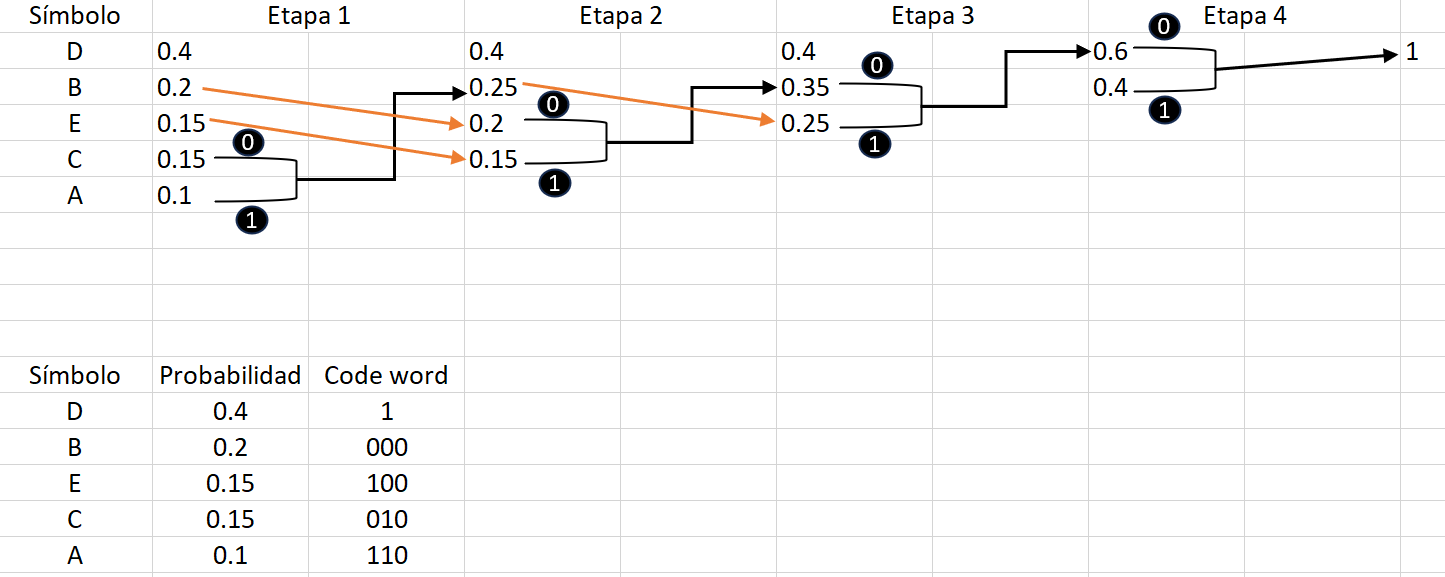
\includegraphics[width=0.8\linewidth]{Captura de pantalla 2025-09-08 164244.png}
    \caption{Diagrama de Huffman}
    \label{fig:placeholder}
\end{figure}

\noindent c) Calcule la longitud media del código. \par
\bigskip
\noindent \begin{equation*}
L = \sum_{i=1}^{n} p_i l_i= \\(0.4 \times 1) + (0.2 \times 3) + (0.15 \times 3) + (0.15 \times 3) + (0.1 \times 3) \\
= 0.4 + 0.6 + 0.45 + 0.45 + 0.3 = 2.2 \text{ bits/símbolo}
\end{equation*}

\noindent d) Calcule la eficiencia del código. \par

\begin{align*}
\eta &= \frac{H(X)}{L} \times 100\% \\
\eta &= \frac{2.146}{2.22} \times 100\% = 97.54\%
\end{align*}

 %   \include{actividad3}
 %   \include{conclusion}
    

%\printbibliography[heading=bibintoc] % Agrega el título "Referencias" al índice automáticamente
    
\end{document}